\documentclass[a4paper,10pt,twoside]{article}

\usepackage[top=1in, bottom=1in, left=1in, right=1in]{geometry}
\usepackage[utf8]{inputenc}
\usepackage[spanish,es-ucroman,es-noquoting]{babel}
\usepackage{setspace}
\usepackage{fancyhdr}
\usepackage{lastpage}
\usepackage{amsmath}
\usepackage{amsfonts}
\usepackage{verbatim}
\usepackage{graphicx}
\usepackage{float}
\usepackage{algorithmic}
\usepackage{tikz}
\usepackage{ gensymb }
\usetikzlibrary{calc}
\usetikzlibrary{decorations.pathreplacing}


% Evita que el documento se estire verticalmente para ocupar
% el espacio vacío en cada página.
\raggedbottom


%%%%%%%%%% Configuración de Fancyhdr - Inicio %%%%%%%%%%
\pagestyle{fancy}
\thispagestyle{fancy}
\lhead{RTP2, Organización del Computador II}
\renewcommand{\footrulewidth}{0.4pt}
\cfoot{\thepage /\pageref{LastPage}}

\fancypagestyle{caratula} {
   \fancyhf{}
   \cfoot{\thepage /\pageref{LastPage}}
   \renewcommand{\headrulewidth}{0pt}
   \renewcommand{\footrulewidth}{0pt}
}
%%%%%%%%%% Configuración de Fancyhdr - Fin %%%%%%%%%%


%%%%%%%%%% Configuración de Algorithmic - Inicio %%%%%%%%%%
% Entorno propio para customizar la presentación del pseudocódigo
\newenvironment{pseudocodigo}
    {\vspace{0.5em} \begin{algorithmic}}
    {\end{algorithmic} \vspace{0.5em}}

% Alinear comentarios a la derecha
\renewcommand{\algorithmiccomment}[1]{\hfill \{#1\}}
%%%%%%%%%% Configuración de Algorithmic - Fin %%%%%%%%%%


%%%%%%%%%% Macros de tikz - Inicio %%%%%%%%%%
% Uso: \registroCuatro{etiqueta}{x}{y}{a4}{a3}{a2}{a1}
\newcommand{\registroCuatro}[7]{
    \ifthenelse{\equal{#1}{}}{}{
        \draw (#2, {#3 + 0.5}) node[anchor=east]{#1};
    }

    \draw   (#2, #3) rectangle +(4, 1) +(2, 0.5) node{#4}
          ++(4, 0)   rectangle +(4, 1) +(2, 0.5) node{#5}
          ++(4, 0)   rectangle +(4, 1) +(2, 0.5) node{#6}
          ++(4, 0)   rectangle +(4, 1) +(2, 0.5) node{#7};          
}

% Uso: \registroOcho{etiqueta}{x}{y}{a8}{a7}{a6}...{a1}
\newcommand{\registroOcho}[9]{
    \def\etiqueta{#1}
    \def\x{#2}
    \def\y{#3}
    \def\aviii{#4}
    \def\avii{#5}
    \def\avi{#6}
    \def\av{#7}
    \def\aiv{#8}
    \def\aiii{#9}
    \registroOchoX    
}
\newcommand{\registroOchoX}[2]{ % Auxiliar - no usar directamente
    \def\aii{#1}
    \def\ai{#2}
    \ifthenelse{\equal{\etiqueta}{}}{}{
        \draw (\x, {\y + 0.5}) node[anchor=east]{\etiqueta};
    }
    \filldraw[fill=white]
        (\x, \y) rectangle +(2, 1) +(1, 0.5) node{\aviii}
        ++(2, 0) rectangle +(2, 1) +(1, 0.5) node{\avii}
        ++(2, 0) rectangle +(2, 1) +(1, 0.5) node{\avi}
        ++(2, 0) rectangle +(2, 1) +(1, 0.5) node{\av}
        ++(2, 0) rectangle +(2, 1) +(1, 0.5) node{\aiv}
        ++(2, 0) rectangle +(2, 1) +(1, 0.5) node{\aiii}
        ++(2, 0) rectangle +(2, 1) +(1, 0.5) node{\aii}
        ++(2, 0) rectangle +(2, 1) +(1, 0.5) node{\ai};
}


% Uso: \registroDieciseis{etiqueta}{x}{y}{a16}{a15}{a14}...{a1}
\newcommand{\registroDieciseis}[9]{
    \def\etiqueta{#1}
    \def\x{#2}
    \def\y{#3}
    \def\axvi{#4}
    \def\axv{#5}
    \def\axiv{#6}
    \def\axiii{#7}
    \def\axii{#8}
    \def\axi{#9}
    \registroDieciseisX
}
\newcommand{\registroDieciseisX}[9]{ % Auxiliar - no usar directamente
    \def\ax{#1}
    \def\aix{#2}
    \def\aviii{#3}
    \def\avii{#4}
    \def\avi{#5}
    \def\av{#6}
    \def\aiv{#7}
    \def\aiii{#8}
    \def\aii{#9}
    \registroDieciseisXX
}
\newcommand{\registroDieciseisXX}[1]{ % Auxiliar - no usar directamente
    \def\ai{#1}
    \ifthenelse{\equal{\etiqueta}{}}{}{
        \draw (\x, {\y + 0.5}) node[anchor=east]{\etiqueta};
    }
    \filldraw[fill=white]
        (\x, \y) rectangle +(1, 1) +(0.5, 0.5) node{\axvi}
        ++(1, 0) rectangle +(1, 1) +(0.5, 0.5) node{\axv}
        ++(1, 0) rectangle +(1, 1) +(0.5, 0.5) node{\axiv}
        ++(1, 0) rectangle +(1, 1) +(0.5, 0.5) node{\axiii}
        ++(1, 0) rectangle +(1, 1) +(0.5, 0.5) node{\axii}
        ++(1, 0) rectangle +(1, 1) +(0.5, 0.5) node{\axi}
        ++(1, 0) rectangle +(1, 1) +(0.5, 0.5) node{\ax}
        ++(1, 0) rectangle +(1, 1) +(0.5, 0.5) node{\aix}
        ++(1, 0) rectangle +(1, 1) +(0.5, 0.5) node{\aviii}
        ++(1, 0) rectangle +(1, 1) +(0.5, 0.5) node{\avii}
        ++(1, 0) rectangle +(1, 1) +(0.5, 0.5) node{\avi}
        ++(1, 0) rectangle +(1, 1) +(0.5, 0.5) node{\av}
        ++(1, 0) rectangle +(1, 1) +(0.5, 0.5) node{\aiv}
        ++(1, 0) rectangle +(1, 1) +(0.5, 0.5) node{\aiii}
        ++(1, 0) rectangle +(1, 1) +(0.5, 0.5) node{\aii}
        ++(1, 0) rectangle +(1, 1) +(0.5, 0.5) node{\ai};
}
%%%%%%%%%% Macros de tikz - Fin %%%%%%%%%%


%%%%%%%%%% Macros misceláneos - Inicio %%%%%%%%%%
\newcommand{\xmm}[1]{\texttt{XMM#1}}
\newcommand{\rax}{\texttt{RAX}}
\newcommand{\rbx}{\texttt{RBX}}
\newcommand{\rcx}{\texttt{RCX}}
\newcommand{\rdx}{\texttt{RDX}}
\newcommand{\rbp}{\texttt{RBP}}
\newcommand{\rsp}{\texttt{RSP}}
\newcommand{\reg}[1]{\texttt{R#1}}
\newcommand{\asm}[1]{\texttt{\uppercase{#1}}}
\newcommand{\INDSTATE}[1][1]{\STATE\hspace{#1\algorithmicindent}}
%%%%%%%%%% Macros misceláneos - Fin %%%%%%%%%%


\begin{document}


%%%%%%%%%%%%%%%%%%%%%%%%%%%%%%%%%%%%%%%%%%%%%%%%%%%%%%%%%%%%%%%%%%%%%%%%%%%%%%%
%% Carátula                                                                  %%
%%%%%%%%%%%%%%%%%%%%%%%%%%%%%%%%%%%%%%%%%%%%%%%%%%%%%%%%%%%%%%%%%%%%%%%%%%%%%%%


\thispagestyle{caratula}

\begin{center}


\includegraphics[height=2cm]{DC.png} 
\hfill

\includegraphics[height=2cm]{UBA.jpg} 

\vspace{2cm}

Departamento de Computación,\\
Facultad de Ciencias Exactas y Naturales,\\
Universidad de Buenos Aires

\vspace{4cm}

\begin{Huge}
RTP2
\end{Huge}

\vspace{0.5cm}

\begin{Large}
Organización del Computador II
\end{Large}

\vspace{1cm}

Primer Cuatrimestre de 2013

\vspace{4cm}

Grupo: \textbf{Panceta y Huevo Frito}

\vspace{0.5cm}

\begin{tabular}{|c|c|c|}
\hline
Apellido y Nombre & LU & E-mail\\
\hline
B\'alsamo, Facundo		& 874/10 & facundobalsamo@gmail.com\\
Gonz\'alez Alba, Pablo	& 476/10 & pablo.gonzalez.alba@gmail.com\\
Lasso, Nicol\'as 			& 763/10 & lasso.nico@gmail.com\\
\hline
\end{tabular}

\end{center}

\newpage


%%%%%%%%%%%%%%%%%%%%%%%%%%%%%%%%%%%%%%%%%%%%%%%%%%%%%%%%%%%%%%%%%%%%%%%%%%%%%%%
%% Índice                                                                    %%
%%%%%%%%%%%%%%%%%%%%%%%%%%%%%%%%%%%%%%%%%%%%%%%%%%%%%%%%%%%%%%%%%%%%%%%%%%%%%%%


\tableofcontents

\newpage


%%%%%%%%%%%%%%%%%%%%%%%%%%%%%%%%%%%%%%%%%%%%%%%%%%%%%%%%%%%%%%%%%%%%%%%%%%%%%%%
%% Introducción                                                              %%
%%%%%%%%%%%%%%%%%%%%%%%%%%%%%%%%%%%%%%%%%%%%%%%%%%%%%%%%%%%%%%%%%%%%%%%%%%%%%%%


\section{Introducción}

El lenguaje C es uno de los más eficientes en cuestión de performance, pero esto no quiere decir que sea óptimo para todos los casos o que no haya campos en los que pueda utilizarse una opción mejor.
Para comprobar esto, experimentamos con el set de instrucciones SIMD de la arquitectura Intel. Vamos a procesar imágenes mediante la aplicación de ciertos filtros y estudiaremos la posible ventaja que puede tener un código en Assembler con respecto a uno en C.
Implementaremos los filtros en ambos lenguajes para luego poder comparar la performance de cada uno y evaluar las ventajas y/o desventajas de cada uno.



%%%%%%%%%%%%%%%%%%%%%%%%%%%%%%%%%%%%%%%%%%%%%%%%%%%%%%%%%%%%%%%%%%%%%%%%%%%%%%%
%% Desarrollo                                                                %%
%%%%%%%%%%%%%%%%%%%%%%%%%%%%%%%%%%%%%%%%%%%%%%%%%%%%%%%%%%%%%%%%%%%%%%%%%%%%%%%


\section{Desarrollo y Resultados}

\subsection{Recortar}

El filtro Recortar únicamente requiere copiar una cantidad $tam$ de píxeles de las esquinas de la imagen fuente para generar la imagen destino con las esquinas invertidas.

\subsubsection{Implementación en C}

Con dos ciclos anidados se recorre el área de $tam$ x $tam$ en cada esquina de la imagen fuente y se escribe en la esquina opuesta de la imagen destino.

\subsubsection{Implementación en Assembler}

También se realiza con dos ciclos anidados, pero trayendo de a 16 píxeles por vez.
En cada iteración se traen 16 píxeles de la parte A a xmm0 con la operación movups y luego se copian a la parte D, lo mismo con 16 píxeles de B en C, de C en B y de D en A. Esto puede verse en el siguiente gráfico.

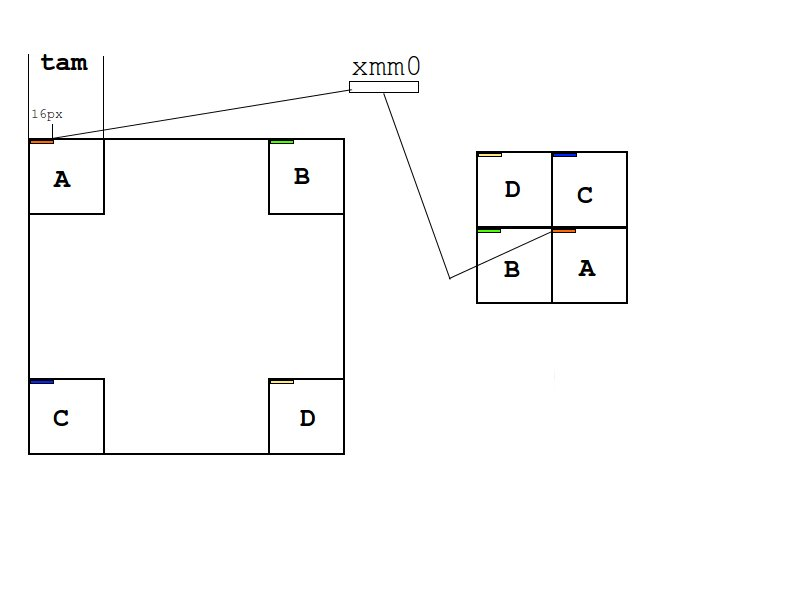
\includegraphics[width=\textwidth]{recortar.jpg} 

En el caso que $tam$ no sea múltiplo de 16, antes de entrar al ciclo se calcula el resto ($tam$ \% 16) y en la primera iteración de cada fila se suma este resto en lugar de los 16 que se suman normalmente. 

\subsubsection{Resultados}

Dado que en este filtro no se modifican los píxeles, la única diferencia debería ser en los accesos a memoria. Los ciclos en ambas implementaciones hacen 8 accesos a memoria, 4 lecturas y 4 escrituras, pero la implementación en ASM accede de a 16 bytes vs 1 de la implementación en C. 
Por lo tanto la ímplementación en C debería ser aproximadamente 16 veces más rápida.

Ejecutamos ambos filtros 1000 veces cada uno y estos son los resultados obtenidos:

\begin{center}
    \begin{tabular}{|l|l|l|}
        \hline
         & Implementación C & Implementación en asm  \\
        \hline
        Duración promedio (en ciclos de clock) & 422 596        & 24 781                 \\
        \hline
    \end{tabular}
\end{center}

Como se puede observar, la implentación en asm es $\sim$17 veces más rápida, lo que corrobora nuestra hipótesis.

\subsection{Halftone}

El filtro Halftone parte a la imagen original en bloques de 2x2 píxeles, se obtiene t como la sumatoria del valor de cada pixel y genera un bloque del mismo tamaño en la imagen destino que cumpla:

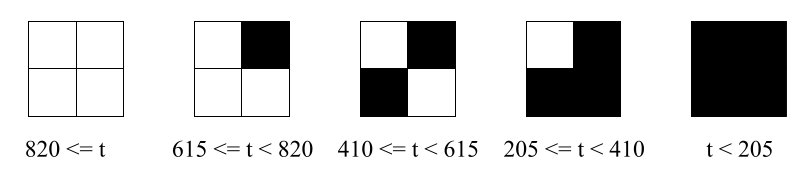
\includegraphics[width=\textwidth]{halftone1.jpg} 

\begin{itemize}
\item El pixel de arriba a la izquierda es blanco si $t \geq$ 205.
\item El pixel de arriba a la derecha es blanco si $t \geq$ 820.
\item El pixel de abajo a la izquierda es blanco si $t \geq$ 615.
\item El pixel de abajo a la derecha es blanco si $t \geq$ 410.
\end{itemize}

Si el ancho y/o alto de la imagen es impar, se descarta la última fila y/o columna, según corresponda.

\subsubsection{Implementación en C}

Con dos ciclos anidados se recorre de 2 en 2 la imagen original.
Se calcula t con la suma de de los valores de los 4 píxeles y luego se setean los píxeles en blanco o negro según corresponda por el valor de $t$.

\subsubsection{Implementación en Assembler}

También se realizan dos ciclos anidados, trayendo cada vez de a 32 píxeles.
Se traen 16 píxeles de la primera línea a xmm0 y 16 de la segunda línea a xmm1.
Como para calcular $t$ se necesita un espacio de más de 1 byte ($t$ puede ser mayor a 255), se desempaquetan y se trabaja primero con los 8 bytes menos significativos, guardando el resto para procesar al terminar estos.
Se suman los 2 registros verticalmente, luego se shiftea un registro para acomodar y volver a sumar.
Esto da como resultado el valor $t$ para cada uno de los 4 bloques como se ve en la siguiente ilustración:

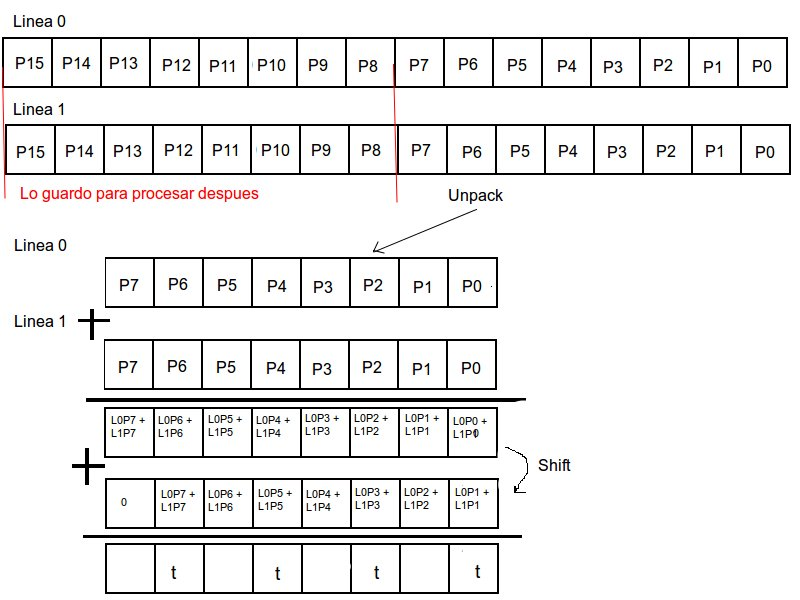
\includegraphics[width=\textwidth]{halftone2.jpg} 

Se compara por mayor o igual en un registro distinto para cada uno de los valores límite.
Luego, ya que  el valor que va a cada pixel es el mismo que el resultado de la comparación (todos 1s o todos 0s), simplemente se ordenan los resultados en los primeros 8 bytes de cada registro.
Se ilustra el proceso para los bytes de la primera línea:

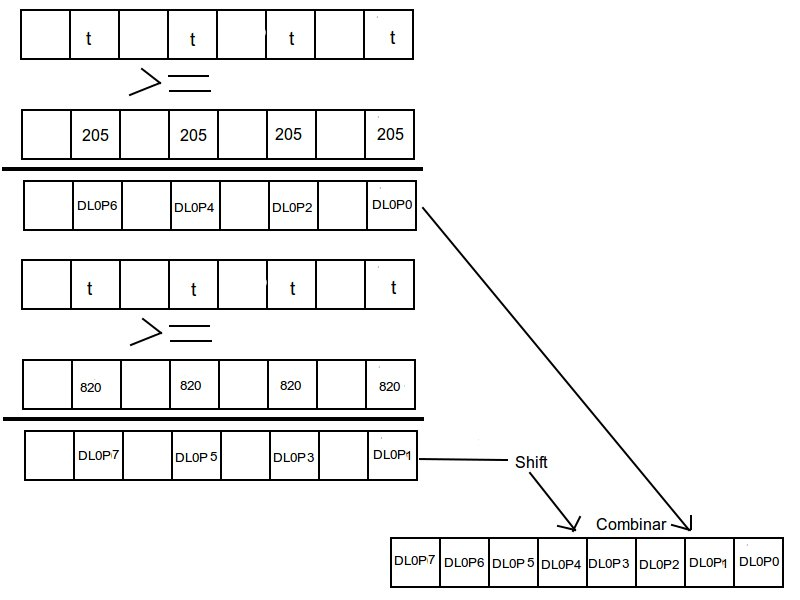
\includegraphics[width=\textwidth]{halftone3.jpg} 

Este proceso se repite con los 8 bytes más significativos que guardamos al principio. Estos resultados se shiftean 8 bytes a la izquieda y combinan (con un $por$) con los primeros resultados, dándonos 2 registros con 16 bytes procesados cada uno, que se copian a la memoria de la imagen destino.

En el caso que el ancho no sea múltiplo de 16, antes de entrar al ciclo se calcula el resto ($width$ \% 16) y en la primera iteración de cada fila se suma este resto en lugar de los 16 que se suman normalmente.

\subsubsection{Resultados}

En la implementación en C, para procesar un bloque de 4 píxeles se requieren 8 accesos a memoria (4 lecturas y 4 escrituras), en cambio en la implementación en ASM, se procesa un bloque de 32 píxeles con tan sólo 4 accesos a memoria.
Con esos datos y, teniendo en cuenta que el acceso a memoria es mucho más lento que cualquier otra operación que se aplique en el filtro, la implementación en ASM debería ser aproximadamente 16 veces más rápida que la implementación en C.

Ejecutamos ambos filtros 1000 veces cada uno y estos son los resultados obtenidos:

\begin{center}
    \begin{tabular}{|l|l|l|}
        \hline
         & Implementación C & Implementación en asm  \\
        \hline
        Duración promedio (en ciclos de clock) & 3 229 822       & 230 612                 \\
        \hline
    \end{tabular}
\end{center}

Como se puede observar, la implentación en asm es $\sim$14 veces más rápida, lo que corrobora nuestra hipótesis.


\subsection{Umbralizar}

Umbralizar es un filtro que debe modificar los píxeles de una imagen en blanco y negro de acuerdo a una fórmula que utiliza ciertos parámetros para calcular el nuevo valor del pixel. El valor inicial del pixel ($I_{pixel}$) y tres enteros (min, max, q), son utilizados para calcular el valor final del pixel (En realidad el valor del nuevo pixel) dada la fórmula siguiente: 0 si $I_{pixel}$ $\textless$  min, 255 si $I_{pixel}$ $\textgreater$ max, $\lfloor$ $I_{pixel}$/q $\rfloor$*q si min $\leq$ $I_{pixel}$ $\leq$ max.

\subsubsection{Implementación en C}

Utilizando dos ciclos anidados que iteren sobre la cantidad de píxeles de alto y de ancho de la imágen, leyendo en cada iteración un pixel, al que se lo procesa según la fórmula ya explicitada.
Una vez procesado, el nuevo valor del pixel es almacenado en la imagen destino.
Cada pixel que se lee implica un acceso a memoria, al igual que cada vez que se guarda el pixel en el destino.

\subsubsection{Implementación en Assembler}

La implementación en ASM sigue la misma lógica que la implementación en C, pero esta vez con la ventaja de poder leer y escribir en una sola iteración 16 pixeles simultaneamente. Eso quiere decir, que por cada acceso a memoria que hacemos en ASM, conseguimos 16 pixeles. Eso mismo en C nos costaría 16 accesos a memoria. Al momento de la escritura sucede lo mismo.


Lo primero que hacemos en ASM es guardar el parámetro q en un registro y expandirlo 4 veces en el mismo (Las instrucciones de las que disponemos nos permiten procesar de a 4 pixeles por vez). También obtenemos otros resultados que utilizaremos para avanzar correctamente por los pixeles que debemos procesar.
Luego de obtener los 16 pixeles a procesar en esta iteracón, se los desempaqueta hasta quedar en grupos de a 4 pixeles por registro. Generamos dos máscaras, una para los menores a min y otra para los mayores a max y luego asignamos el valor 0 a los pixeles menores a min.


Para procesar correctamente los pixeles, deben ser convertidos a float antes de la división, y  reconvertilos a int para asegurar que sólo contengan la parte entera de la división antes de multiplicar. De nuevo hay que convertirlos a float y finalmente multiplicar por Q. Una vez hecha la multiplicacion, utilizamos una de las máscaras obtenidas anteriormente para que en los píxeles mayores a max tengan un 1 en cada bit.


Este proceso debe ser repetido 4 veces por ciclo ya que si bien se puede leer 16 píxeles en cada iteración, las instrucciones solo me permiten procesar de a 4. Por este motivo debemos luego volver a empaquetar los píxeles hasta que nos quede en un registro, los 16 píxeles procesados. Debemos tener en cuenta al empaquetar, que la instrucción PACKUSWB, que usamos para empaquetar dos registros con 8 int cada uno en un registro con 16 int, asume que los valores que contienen los registros son signed int. Esto quiere decir que al empaquetar, va a transformar a 0 los píxeles cuyo bit más significativo es un 1 (Por ejemplo los píxeles que eran mayores a max). Para solucionar esto, antes de realizar el empaquetado, transformamos el bit más significativo en 0 para cada píxel.


Los últimos dos pasos son escribir en la imágen destino los nuevos 16 píxeles con un solo acceso a memoria y avanzar a los próximos píxeles a procesar si correspondiera o terminar la ejecución si ya fueron procesados todos los píxeles.

\subsubsection{Resultados}

En la implementación C podemos leer de a un píxel por cada acceso a memoria, a diferencia de la implementación ASM que permite leer 16 píxeles en cada iteración. Por este motivo podríamos a priori suponer que el código asm debería ser 16 veces más rápido que el correspondiente código en C.

Ejecutamos ambos filtros 1000 veces cada uno y estos son los resultados obtenidos:

\begin{center}
    \begin{tabular}{|l|l|l|}
        \hline
         & Implementación C & Implementación en asm  \\
        \hline
        Duración promedio (en ciclos de clock) & 6 252 872        & 1 001 096 \\
        \hline
    \end{tabular}
\end{center}

Como se puede observar, la implentación en asm es apenas $\sim$6 veces más rápida.
 
 
La razón de la diferencia entre la hipótesis y el resultado obtenido la podemos ver en lás operaciones realizadas para procesar los píxeles. Si bien corremos con la ventaja de que el código ASM hace un llamado a memoria por cada 16 que realiza el código C, no podemos procesar los 16 píxeles simultaneamente sino que podemos hacerlo de a 4. Además existe el costo de desempaquetar y empaquetar reiteradas veces a lo largo de cada iteración del ciclo, con lo cual la ventaja sobre el código C se ve reducida. La generación de las máscaras y su aplicación, también colaboran para nivelar la diferencia entre ambos códigos.


A favor de la implementación en ASM, podemos ver que no sólo accedemos menos veces a memoria a la hora de leer píxeles, sino que también podemos, antes de entrar a los ciclos, guardar en registros algunos valores que el código C buscaría en cada iteración dentro de la memoria, como por ejemplo $max$ o $Q$.

\subsection{Colorizar}

El filtro Colorizar resalta los colores de la imagen de acuerdo al color predominante en un bloque de 3x3 píxeles según la siguiente regla:

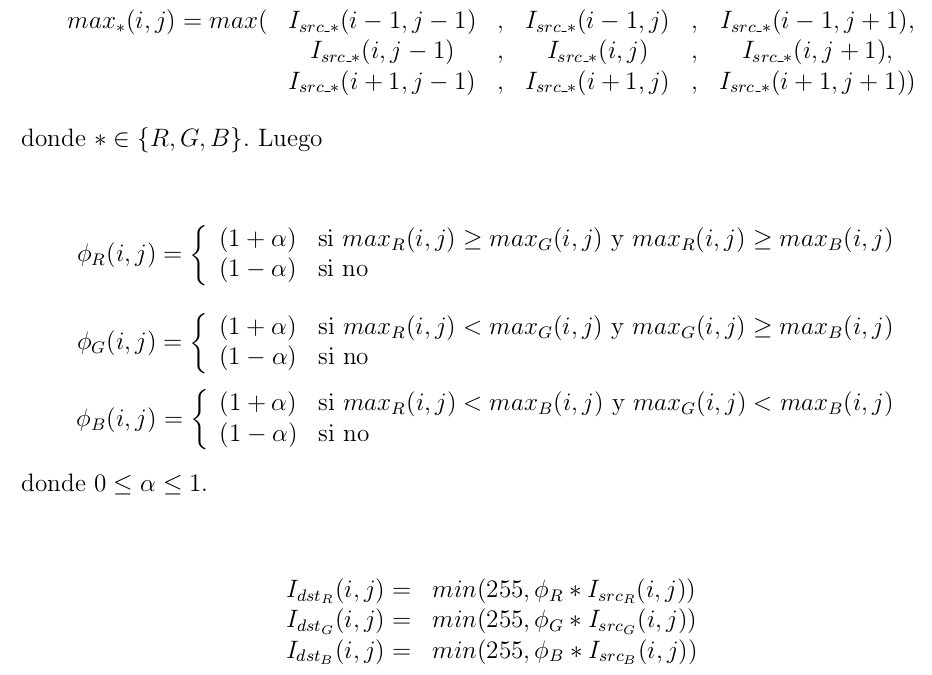
\includegraphics[width=\textwidth]{colorizar.jpg} 

\subsubsection{Implementación en C}

Se recorre la imagen con dos ciclos anidados de pixel en pixel (3 bytes) ignorando la primer y última fila y columna, calculando el valor de cada color del pixel destino.
Para calcular ese valor hay una función para el menor, mayor y $\phi$, lo que hace que además de traer los 8 píxeles que lo rodean, se hagan 15 llamados a funciones con su correspondiente costo de acceso a memoria.

\subsubsection{Implementación en Assembler}

En este filtro, como cada pixel ocupa 3 bytes y requiere tener datos de su predecesor y siguiente, se traen de a 5 píxeles y se ignora un byte.
Como en los demás filtros se hacen 2 ciclos anidados pero con ciertos detalles:
\begin{itemize}
\item En la altura empieza en 0 y va hasta height - 2, ya que en cada iteración se traen 3 filas.
\item En el ancho se trae primero desde el 0 y se ignora el último byte, pero en las siguientes iteraciones se ignora el primer byte, esto es para evitar pasarse y traer bytes que no pertenezcan a la imagen.
\item Al escribir en el destino, se escriben solamente 9 bytes nuevos (3 bytes), estos se colocan en la parte más significativa para no pasarse al escribir los bytes. Por esto se deben guardar los últimos 7 bytes de la iteración anterior para completar el registro y no pisar datos ya procesados.
\end{itemize}

En cada iteración se traen 16 bytes en 3 registros para tener suficiente como para procesar 3 píxeles.
El método para procesar 1 pixel consiste en calcular los máximos, luego comparar, calcular $\phi$ y, por último, multiplicar por $\pm$ $\alpha$ según corresponda:

\begin{pseudocodigo}
	\STATE maximos(regSrc, regDst) \{
	\INDSTATE[2] $regSrc = \{Basura, p1b, p1g, p1r, p2b, p2g, p2r, p3b, p3g, p3r, Basura, Basura, Basura, Basura, Basura, Basura\}$
	\INDSTATE[2] xmm3 = unpackLower(regSrc)
	\INDSTATE[2] xmm4 = unpackLower(xmm3)
	\INDSTATE[2] xmm5 = unpackLower(shiftRight(xmm3, 6))
	\INDSTATE[2] xmm4 = max(xmm4, xmm5)
	\INDSTATE[2] xmm3 = unpackLower(unpackLower(shiftRight(regSrc, 6)))
	\INDSTATE[2] regDst = max(xmm4, xmm3) \COMMENT{regDst = $\{Basura, MaxB, MaxG, MaxR\}$}
    \STATE \}
\end{pseudocodigo}

\begin{pseudocodigo}
	\STATE maximos(regLinea0, xmm6)
	\STATE maximos(regLinea1, xmm7)
	\STATE xmm6 = max(xmm6, xmm7)
	\STATE maximos(regLinea2, xmm7)
	\STATE xmm6 = (float) max(xmm6, xmm7) \COMMENT{xmm4 = $\{Basura, MaxB9, MaxG9, MaxR9\}$}
	\STATE pixelActual = (float) unpackHigher(unpackLower(regLinea1)) \COMMENT{Valores del pixel actual}
	
	\COMMENT{Hago shuffle para que me queden alineados y comparo}
	\STATE xmm6 = $\{Basura, MaxR, MaxG, MaxR\}$
	\STATE xmm7 = $\{Basura, MaxB, MaxB, MaxG\}$
	\STATE xmm8 = xmm6 $\geq$ xmm7
	\STATE $\phi$R = maxR $\geq$ maxG $\land$ maxR $\geq$ maxB
	\STATE $\phi$G = maxR $\textless$ maxG $\land$ maxG $\geq$ maxB
	\STATE $\phi$B = maxR $\textless$ maxB $\land$ maxG $\textless$ maxB
	\STATE reg$\phi$ = $\{Basura, \phi$B, $\phi$G, $\phi$R $\}$
	\STATE signo = reg$\phi$ $\land$ 0x80000000800000008000000080000000
	\STATE reg$\alpha$ = $\{ Basura, \alpha, \alpha, \alpha\}$
	\STATE signed$\alpha$ = reg$\alpha$ $\land$ $\neg$ signo \COMMENT{Queda $\alpha$ negativo en donde no se cumpla $\phi$}
	\STATE dst = pixelActual + pixelActual * signed$\alpha$ \COMMENT{Equivalente a pixelActual * (1 $\pm$ $\alpha$)}
	
\end{pseudocodigo}

Esto se repite para los otros 2 píxeles que puedo procesar por iteración y se acomodan, primero los 7 valores más significativos de la iteración anterior y luego los 9 bytes nuevos para escribir en la imagen destino.

\subsubsection{Resultados}

En la implementación en C, debido a los píxeles vecinos y las llamadas a funciones, se realizan, al menos, 25 accesos a memoria por cada pixel en la imagen destino.
En cambio en la implementación en ASM, para un bloque de 3 píxeles se realizan 4 accesos a memoria, 3 lecturas y una escritura. Por lo tanto debería ser al menos 18 veces más rápido.

Ejecutamos ambos filtros 100 veces cada uno y estos son los resultados obtenidos:

\begin{center}
    \begin{tabular}{|l|l|l|}
        \hline
         & Implementación C & Implementación en asm  \\
        \hline
        Duración promedio (en ciclos de clock) & 556 480 896        & 13 323 085 \\
        \hline
    \end{tabular}
\end{center}

Como se puede observar, la implentación en asm es $\sim$42 veces más rápida, lo que corrobora la hipótesis. La mejora mucho más significativa podemos verla analizando el código ASM generado por el gcc:
Variables locales auxiliares generan muchos más accesos a memoria por función, cosa que en el código ASM evitamos completamente sabiendo que pueden realizarse únicamente con registros.

\subsection{Efecto Plasma}

La función waves consiste en generar unas ondas sobre la imagen destino, aplicando a cada pixel de la imagen fuente, la siguiente función:

$prof_{i,j}$ =
$(x_{scale} * sin\_taylor(i / 8.0) + y_{scale} * sin\_taylor(j / 8.0)) / 2$

$I_{dest}$(i, j) = $prof_{i,j}$ * $g_{scale}$ + $I_{src}$(i, j)

Además $I_{dest}$(i, j) debe guardarse como 0 ó 255, si este sobrepasa el intervalo [0, 255].

\subsubsection{Implementación en C}

Se crea una función particular para calcular el sin\_taylor.
Con 2 ciclos anidados se recorren todos los píxeles de la imagen fuente, se calculan los sin\_taylor y se multiplican por las scale correspondientes. Luego se suma al valor del pixel fuente, se coloca dentro del intervalo [0, 255] y se guarda en la imagen destino.

\subsubsection{Implementación en Assembler}

El sin\_taylor se calcula con una macro, para evitar definir nuevas funciones y sus cargas en accesos a memoria, pero manteniendo el código en un solo lugar. Este mismo concepto está aprovechado por muchos compiladores y se conoce como function inlining (se copia el código de la función en todos los lugares dónde es llamada).
Esta macro además hace la división por 8 y multiplica por el scale correspondiente, como puede verse en este pseudo-código:

\begin{pseudocodigo}
	\STATE $Prerequisito: xmm0 = \{i, i, i, i\}$ \COMMENT{con i el parámetro a aplicar sin\_taylor()}
	\STATE scale\_sin\_taylor\_div\_8(scale) \{
    		\INDSTATE[2] xmm0 = xmm0 / 8
    		\INDSTATE[2] xmm1 = xmm0 \COMMENT{xmm1 = xmm0 = $\{i/8, i/8, i/8, i/8\}$}
    		\INDSTATE[2] xmm0 = $\lfloor$xmm0 / 2 $\pi\rfloor$ * 2 $\pi$
    		\INDSTATE[2] xmm0 = xmm1 - xmm0 - $\{\pi, \pi, \pi, \pi\}$
    		\INDSTATE[2] xmm0 = xmm0 - xmm0$^{3}$ / 6 + xmm0$^{5}$ / 120 - xmm0$^{7}$ / 5040
    		\INDSTATE[2] xmmo = xmm0 * $\{scale, scale, scale, scale\}$
    \STATE \}
\end{pseudocodigo}

El filtro en sí se realiza con dos ciclos anidados trayendo de a 16 píxeles por vez.
El sin\_taylor de la altura se calcula una sola vez por iteración en las filas y se guarda para evitar repetir cálculos.
El ciclo trae 16 píxeles, pero procesa de a 4 y los va uniendo al final como indica el siguiente pseudo-código:

\begin{pseudocodigo}
	\STATE i = j = 0
	\STATE checkearResto = resto = width \% 16
	\WHILE{i $\textless$ height}
		\STATE xmm0 = $\{i, i, i, i\}$
		\STATE xmm5 = scale\_sin\_taylor\_div\_8(y\_scale)
		
		\WHILE{j $\textless$ width}
			\STATE xmm12 = *(pointerSrc + i * src\_row\_size + j) \COMMENT{16 píxeles}
			\STATE tmp = j
			
			\FOR{k in [1..4]}
				\STATE xmm4 = unpackLower(unpackLower(xmm12)) \COMMENT{xmm4 = $\{p0, p1, p2, p3\}$}
				\STATE xmm0 = $prof_{i,j}$(tmp, xmm5)
				\STATE xmm0 = (int) (xmm0 + xmm4)
				\STATE xmm0 = packSaturando(packSaturando(xmm0)) \COMMENT{xmm0 = $\{dst_{p0}, dst_{p1}, dst_{p2}, dst_{p3}\}$}
				\STATE xmm12 = xmm0[0..3] + xmm12[4..15]
				\STATE rotar(xmm12, 4) \COMMENT{Roto para en la siguiente iteración trabajar con otros píxeles y que al final quede ordenado de nuevo}
				\STATE tmp += 4
			\ENDFOR
			
			\STATE *(pointerDst + i * src\_row\_size + j) = xmm12 \COMMENT{16 píxeles}
			\IF{checkearResto}
				\STATE j += resto
				\STATE checkearResto = false
			\ELSE
				\STATE j += 16
			\ENDIF
		\ENDWHILE
		\STATE i++
		\STATE checkearResto = true
	\ENDWHILE
	
	\STATE $prof_{i, j}$(i, sin\_taylor\_j) \{
		\INDSTATE[2] xmm0 = (float) $\{i, i+1, i+2, i+3\}$
		\INDSTATE[2] xmm0 = scale\_sin\_taylor\_div\_8(x\_scale)
		\INDSTATE[2] xmm0 = g\_scale * (sin\_taylor\_j + xmm0) / 2
	\STATE \}
\end{pseudocodigo}

En el caso que ancho de la imagen no sea múltiplo de 16, antes de entrar al ciclo se calcula el resto (width \% 16) y en la primera iteración de cada fila se suma este resto en lugar de los 16 que se suman normalmente. 

\subsubsection{Resultados}

En la implementación en C, para procesar un bloque de 1 pixel se requieren 2 accesos a memoria para la lectura y escritura, pero además hace 2 llamadas a una función que, a su vez, hace 4 llamadas más, al menos 10 accesos a memoria más.
En cambio en la implementación en ASM, se procesa un bloque de 16 píxeles con tan sólo 2 accesos a memoria. La implementación en ASM debería ser aproximadamente 96 veces más rápida.

Ejecutamos ambos filtros 100 veces cada uno y estos son los resultados obtenidos:

\begin{center}
    \begin{tabular}{|l|l|l|}
        \hline
         & Implementación C & Implementación en asm  \\
        \hline
        Duración promedio (en ciclos de clock) & 557 984 064        & 5 525 040 \\
        \hline
    \end{tabular}
\end{center}

Como se puede observar, la implentación en asm es $\sim$101 veces más rápida, lo que corrobora la hipótesis y muestra la gran diferencia que genera acceder a funciones dentro de cada iteración del ciclo.

\subsection{Rotar}

El objetivo del algoritmo es rotar la imagen 45$\degree$ hacia la izquierda (sentido antihorario) utilizando la siguiente fórmula:

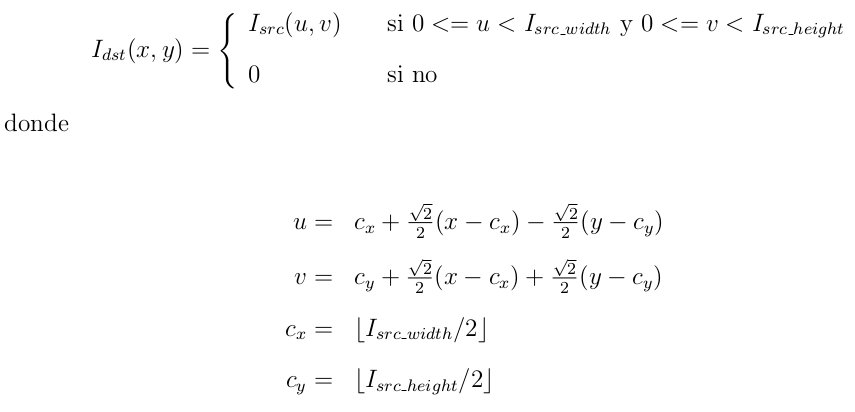
\includegraphics[width=\textwidth]{rotar.jpg} 

\subsubsection{Implementación en C}

La implementación es muy directa con respecto a la especificación. Dos ciclos anidados para recorrer los píxeles destino, y dentro de cada iteración se calculan $u$ y $v$ y se define si se debe colocar un pixel negro o el valor de $I_{src}$(u, v).
Para cada pixel se realiza uno o dos accesos a memoria según corresponda leer o no.

\subsubsection{Implementación en Assembler}

Este filtro tiene ciertas características que impiden aprovechar las operaciones SIMD:
\begin{itemize}
\item Primero, el cálculo de $u$ y $v$ depende de la posición horizontal en la imagen, por lo tanto para calcular 16 píxeles se requieren 16 valores distintos. Esto hace perder la ventaja de realizar varias operaciones en simultáneo ya que cargar 16 valores distintos y luego calcular una sola vez tiene un costo similar a calcular 16 veces. Sin embargo, podría realizarse igualmente (de hecho, algo similar sucede con el filtro waves) de no ser por:
\item Los valores de píxeles consecutivos de la imagen destino dependen de píxeles no consecutivos en la imagen fuente, como puede observarse fácilmente en la imagen de ejemplo. En consecuencia, para escribir 16 píxeles se requiere de 16 lecturas independientes a memoria, arruinando la principal ventaja que estábamos obteniendo con operaciones SIMD.
\end{itemize}

El filtro Rotar, por su forma que lo caracteriza, es incapaz de aprovechar los registros $xmm$ para acceder a memoria efectivamente. Y, aunque por medio dea microoptimizaciones, como prescindir de variables locales en memoria, se podría obtener un mejor resultado que en la versión en C, lo que vimos en los otros filtros demuestra que el principal factor en determinar la eficacia eran los accesos a memoria y cualquier mejora sería despreciable.
Por lo tanto decidimos no implementarlo.



%%%%%%%%%%%%%%%%%%%%%%%%%%%%%%%%%%%%%%%%%%%%%%%%%%%%%%%%%%%%%%%%%%%%%%%%%%%%%%%
%% Conclusión                                                                %%
%%%%%%%%%%%%%%%%%%%%%%%%%%%%%%%%%%%%%%%%%%%%%%%%%%%%%%%%%%%%%%%%%%%%%%%%%%%%%%%


\section{Conclusión}

Las instrucciones SIMD (Single Instruction Multiple Data) proveen al programador de una herramienta más efectiva para realizar el mismo conjunto de operaciones a una gran cantidad de datos.

La aplicación del filtros a imágenes era un ejemplo perfecto para probar su eficiencia.

Analizando los resultados de las implementaciones de los 6 filtros, podemos notar:

\begin{itemize}
\item Las operaciones básicas (padd, psub, pmul, pdiv, shifts, etc.) SIMD tienen un costo similar a sus correspondientes operaciones unitarias, pero generalmente requieren algún tipo de preproceso para poder trabajar con los 16 bytes (pack, unpack, shifts) en una sola iteración, por lo tanto, aunque más eficientes, no lo son en una relación directamente proporcional.
\item En el caso que sí hay una relación directamente proporcional es en el acceso a memoria (como se comprobó en el filtro recortar).
\item Además, el acceso a memoria es, por lejos, la operación más costosa de las que implementamos en cada filtro.
\item Por consecuencia directa del ítem anterior, las llamadas a otras funciones (que a su vez, probablemente contengan variable locales) dentro de una iteración provocan estragos en la efectividad de las implementaciones en C.
\item Para poder aprovechar las instrucciones SIMD es un prerequisito que los datos estén contiguos en memoria. Como descubrimos con el filtro Rotar, los datos dispersos nos obligan a hacer múltiples lecturas a memoria y perder tiempo reordenándolos dentro de los registros antes de poder procesarlos.
\end{itemize}

Concluimos que, definitivamente, las instrucciones SIMD, cuando pueden aprovecharse, demuestran una gran eficiencia. Sin embargo, hay que tener algunas consideraciones:

Aunque las imágenes, video y sonido son los primeros candidatos a ser optimizados por paralelización, no todos los procesos pueden ser efectivos y se requiere un análisis profundo de los datos para ver si vale el esfuerzo.

Además, aunque se pueda lograr una gran optimización, no siempre es lo más importante. Ninguno de los filtros implementados demoró más de 1 segundo en ejecutarse completamente. La optimización seguramente es indispensable en transmisiones de video en vivo, pero baja en importancia si tuviese que ser aplicado una sola vez en una aplicación tipo MS Paint.

Las desventajas que podrían opacar a la optimización son:

El código no es portable, únicamente funciona en procesadores que implementan el set de instrucciones AMD64, requiriendo reescrituras para otras plataformas. Sin embargo el código C debería funcionar perfectamente en IA-32, ARM y cualquier otro procesador que tenga un compilador de lenguaje C.

El código es mucho más largo y difícil de entender (por lo tanto mayor posibilidad de tener bugs) que en un lenguaje de más alto nivel como C. Y en pos de la optimización, se llegan a eliminar funciones (poniéndolas inline), lo que genera código repetido, largo y confuso.




\end{document}